\documentclass{article}
\usepackage[T1]{fontenc}
% DOC PRE-AMBLE
\usepackage[a4paper,margin={1in,1in}]{geometry}
\usepackage{hyperref}
\usepackage{url}
\usepackage{graphicx}
\title{MPHYG001 Assignment 2: Refactoring Boids}
\author{\\
Danial Dervovic\\
\normalsize University College London\\
\normalsize \href{mailto:danial.dervovic.11@ucl.ac.uk}{\texttt{danial.dervovic.11@ucl.ac.uk}}
}
% CODE PRE-AMBLE
\usepackage{listings}
\lstset{language=bash, basicstyle=\ttfamily\footnotesize, keepspaces=true
showspaces=false,breaklines=true, showstringspaces=false, frame=single,
upquote=true}


\begin{document}
\maketitle
\section*{Introduction/Usage}
For this assignment, the task was to take the Boids code\footnote{\href{http://development.rc.ucl.ac.uk/training/engineering/ch05construction/10boids.html}{\texttt{http://development.rc.ucl.ac.uk/training/engineering/ch05construction/10boids.html}}}, packaging it up into a form that can be \texttt{pip} installed and run from the command line. This code may be found at the GitHub repository \href{https://github.com/ddervs/bad-boids}{\texttt{ddervs/bad-boids}}. The usage of the packaged function is shown below (the output of \texttt{boids -{}-help}).
\begin{lstlisting}
usage: boids [-h] [--config CONFIG] [--example_config]

Runs the boids simulation.

optional arguments:
  -h, --help        show this help message and exit
  --config CONFIG   YAML file with simulation options. See README.md or use
                    --example-config option for specification.
  --example_config  Saves default config file to current working directory.
\end{lstlisting}
\section*{Refactorings}
In this task, the refactoring approach was used. The common refactorings utilised in the code are shown in the table below.
\begin{center}
\begin{tabular}{|c|c|}
    \hline
    \textbf{Code Smell} & \textbf{Commit number} \\
    \hline\hline
    Repeated Loops & \texttt{515da7c} \\
    Magic Numbers & \texttt{87c90c7} \\
    Turn \texttt{boids} into a class & \texttt{2ff425b} \\
    Repeated code/copypasta & \texttt{0128753} \\
    Many constants $\rightarrow$ config file & \texttt{a23e2fa} \\
    Large function into units & \texttt{fa117b3} \\
    Too many loops $\rightarrow$ \texttt{numpy} & \texttt{980ce16} \\
    \hline
\end{tabular}
\end{center}
The main advantage of such an approach is that at each stage, the code set still works as originally. This contrasts with the approach of rewriting code, which is both more bug-prone, and requires significant time until the new working code set makes itself available. Refactoring stops code from \emph{rotting} without breaking it, both in the sense of ensuring it is resistant to new developments in the environment of its dependencies, and keeping it readable for future maintenance. The UML diagram for the \texttt{boids} package is shown in Figure~\ref{fig:UML}.
\begin{figure}
\centering
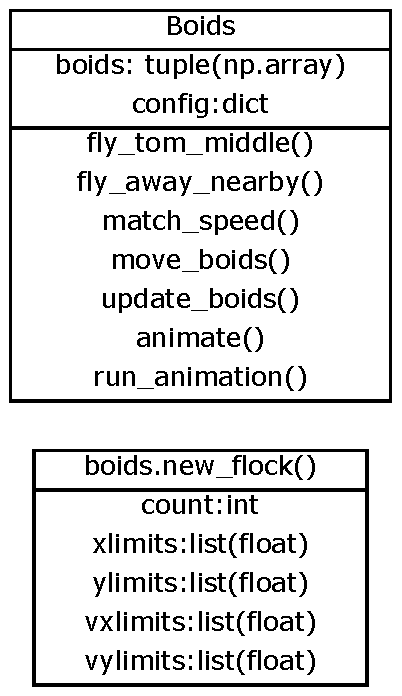
\includegraphics[width=0.25\linewidth]{UML}
\caption{UML diagram of \texttt{boids} package.}
\label{fig:UML}
\end{figure}
\section*{Problems}
The main problems encountered in the project were in integrating the configuration file with the command line interface, and in plotting the animation.
\par
It was found that in \texttt{setup.py}, it was needed to specify the fact that there was a non-python config file in the package. This was because under \texttt{pip} installation, only python files are installed by default. Thus, when the config file was imported in the code, it would only work when executed in the package's root directory.
\par
Another big problem was plotting the animation. The main issue is discussed at \url{http://stackoverflow.com/questions/21099121/python-matplotlib-unable-to-call-funcanimation-from-inside-a-function} and \href{https://github.com/matplotlib/matplotlib/issues/1656}{\texttt{matplotlib issue \#1656}}. For certain GUI backends, if the animation isn't stored in a persistent variable, it will quietly fail, as python's garbage collection will clear the plot. Thus the command line entry point scripts had to be restructured (commit \texttt{eecacbf}) to avoid this happening.


\end{document}
